\documentclass[UTF8]{ctexart}
\usepackage{xcolor}
\usepackage{enumerate}
\usepackage{graphicx}
\usepackage{geometry}
\usepackage{graphicx} %插入图片的宏包
\usepackage{float} %设置图片浮动位置的宏包
\usepackage{subfigure} 
\usepackage[colorlinks,linkcolor=blue]{hyperref}
\usepackage{mathtools}
\usepackage{listings}
\lstset{ %
    language=python,                % the language of the code
    basicstyle=\footnotesize,           % the size of the fonts that are used for the code
    numbers=left,                   % where to put the line-numbers
    numberstyle=\tiny\color{gray},  % the style that is used for the line-numbers
    stepnumber=2,                   % the step between two line-numbers. If it's 1, each line 
                                    % will be numbered
    numbersep=5pt,                  % how far the line-numbers are from the code
    backgroundcolor=\color{white},      % choose the background color. You must add \usepackage{color}
    showspaces=false,               % show spaces adding particular underscores
    showstringspaces=false,         % underline spaces within strings
    showtabs=false,                 % show tabs within strings adding particular underscores
    frame=single,                   % adds a frame around the code
    rulecolor=\color{black},        % if not set, the frame-color may be changed on line-breaks within not-black text (e.g. commens (green here))
    tabsize=2,                      % sets default tabsize to 2 spaces
    captionpos=b,                   % sets the caption-position to bottom
    breaklines=true,                % sets automatic line breaking
    breakatwhitespace=false,        % sets if automatic breaks should only happen at whitespace
    title=\lstname,                 % show the filename of files included with \lstinputlisting;
                                    % also try caption instead of title
    keywordstyle=\color{blue},          % keyword style
    commentstyle=\color{green},       % comment style
    stringstyle=\color{red},         % string literal style
    escapeinside={\%*}{*)},            % if you want to add LaTeX within your code
    morekeywords={*,...}               % if you want to add more keywords to the set
}
\geometry{left = 2.5cm,right= 2cm}
\title{Chapter 3 \\Classification}
\author{DuLi}
\date{\today}
\begin{document}
\maketitle
\newpage
\tableofcontents
\newpage
第一章我们提到过,监督学习中最常见的任务是回归问题(预测)和分类问题。第二章我们探索了回归问题,这一章我们重点关注分类问题。
\section{MNIST}
\setlength{\parskip}{0.5em} 

In this chapter,we will be using the MNIST dataset,which is a set of 70000 small images of digits handwritten by high school students and employees of the US Census Bureau.Each image is labeled with the digit it represents.这个数据集经常被当作Machine Learning中的Hello World问题:这个数据集也经常被用来测试一个新的分类算法。

Scikit-Learn provides many helper functions to download popular datasets.MNIST is one of them.The following code fetches the MNIST dataset:

\begin{lstlisting}
from sklearn.datasets import fetch_mldata

mnist = fetch_mldata('MNIST original',data_home='./')
mnist
\end{lstlisting}
不知道为什么,下载一直有问题,远程连接关闭,所以直接下载下来放在文件夹就OK了。

\begin{figure}[H]
\centering
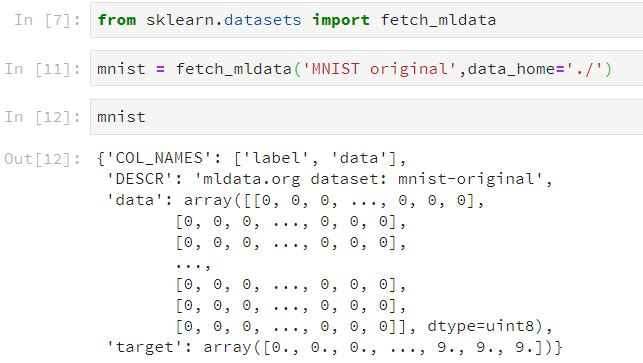
\includegraphics[width = 4in]{mnist_download.JPG}
\caption{Overview of the MNIST dataset}
\end{figure}

先简单说一下数据集的结构:
\begin{itemize}
	\item DESCR关键字存储的是数据集的描述。也就是一句话,mldata.org dataset:mnist-original.
	\item data关键字储存的一行一行的数据,每一行存储一个字符的像素.
	\item target关键字保存的是对应列代表的数字。
\end{itemize}

There are 70,000 images and each image has 784 features(28*28=784 pixels),and each feature simply represents one pixel's intensity ,from 0(white) to 255(black).Let's take a peek at one digit from the dataset.We grab the vector and reshape it to a 28X28 array.

\begin{lstlisting}
X,y = mnist['data'],mnist['target']

import matplotlib
import matplotlib.pyplot as plt

some_digit = X[1123]
some_digit_image = some_digit.reshape(28,28)

plt.imshow(some_digit_image,cmap=matplotlib.cm.binary,interpolation="nearest")
plt.axis("off")
plt.show()
\end{lstlisting}

\begin{figure}[H]
\centering

\includegraphics[width = 2in]{some_digit.JPG}
\caption{Random digits in the data set}
\end{figure}
很明显,这是一个0,值得注意的是,MNIST数据集已经分割好了训练集和测试集,分别是前60000和后10000张图像。

\begin{lstlisting}
X_train,X_test,y_train,y_test = X[:60000],X[60000:],y[:60000],y[60000,]
\end{lstlisting}

同时,我们还要shuffle数据集。主要原因在于这样在做cross-vaildation的时候,可以让每一次fold都很接近。并且,一些算法对于训练集的先后顺序是敏感的,如果连续的输入相同的训练集将会影响算法的性能。

\begin{lstlisting}
import numpy as np

shuffle_index = np.random.permutation(60000)
X_train,y_train = X_train[shuffle_index],y_train[shuffle_index]
\end{lstlisting}

\section{Training a Binary Classifier}

\end{document}
